\documentclass[a4paper]{article}
%\usepackage[affil-it]{authblk}
\usepackage[backend=bibtex,style=numeric]{biblatex}
\usepackage{graphicx}
\usepackage{amsmath}
\usepackage{geometry}
\usepackage{caption}
\usepackage{amssymb}
\usepackage{float}
\usepackage{ctex}
\geometry{margin=1.5cm, vmargin={0pt,1cm}}
\setlength{\topmargin}{-1cm}
\setlength{\paperheight}{29.7cm}
\setlength{\textheight}{25.3cm}

\begin{document}
% ==================================================
\title{Numerical Analysis Homework 3}

\author{罗开诚 3220103383
  \thanks{Electronic address: \texttt{3220103383@zju.edu.com}}}
%\affil{(Information and Computational Science 2201), Zhejiang University}

\date{Due time: \today}

\maketitle

\begin{abstract}
    Solutions to various numerical analysis problems.
\end{abstract}

% ============================================

\section*{Exercise 4.33}
\begin{align*}
  (i) & \quad b \gets 8.769 \times 10^4 ; \quad e_c \gets 4 \\
  (ii) & \quad m_c \gets 10.003 \\
  (iii) & \quad m_c \gets 1.0003 ; \quad e_c \gets 5 \\
  (iv) & \quad \text{do nothing} \\
  (v) & \quad m_c \gets 1.000 \\
  (vi) & \quad c \gets 1.000 \times 10^5 \\
\end{align*}
\begin{align*}
    (i) & \quad b \gets -0.0005678 \times 10^4 ; \quad e_c \gets 4 \\
    (ii) & \quad m_c \gets 1.2334322 \\
    (iii) & \quad \text{do nothing} \\
    (iv) & \quad \text{do nothing} \\
    (v) & \quad m_c \gets 1.233 \\
    (vi) & \quad c \gets 1.233 \times 10^4 \\
\end{align*}
\begin{align*}
  (i) & \quad b \gets -0.5678 \times 10^4 ; \quad e_c \gets 4 \\
  (ii) & \quad m_c \gets 0.6662 \\
  (iii) & \quad m_c \gets 6.662 ; \quad e_c \gets 3 \\
  (iv) & \quad \text{do nothing} \\
  (v) & \quad m_c \gets 6.662 \\
  (vi) & \quad c \gets 6.662 \times 10^3 \\
\end{align*}

\section*{Exercise 4.42}
example:\\
  in FPN (3,3,10,-10)\\

consider $2*3^{0}+1*3^{4}+1.11*3^{2}$\\

use this order to calculate $2*3^{0}+1*3^{4}=1.00*3^{4}$, $1.00*3^{4}+1.11*3^{2}=fl(1.00111*3^4)=1.00*3^4$\\
corresponding $|\delta|=0.15625$\\
change the order after sorting\\
$2*3^{0}+1.11*3^{2}=1.20*3^2$, $1.20*3^2+1*3^{4}=fl(1.012*3^{4})=1.02*3^{4}$\\
corresponding $|\delta|=0.03125$\\
effectively reduced the error\\

\section*{Exercise 4.43}
Based on Lemma 4.34, for \( a, b \in \mathcal{F} \), \( fl(a+b) = (a+b)(1+\delta) \), where \( \delta < \epsilon_u \). By applying this three times, we get:\\

\[ = fl((a_1b_1)(1+\delta_1) + (a_2b_2)(1+\delta_2) + (a_3b_3)(1+\delta_3) + (a_4b_4)(1+\delta_4)) \]
According to Theorem 4.41, this can be further expressed as:\\
\[ = (1+\delta_5)((a_1b_1 + a_2b_2 + a_3b_3 + a_4b_4) + (\delta_1a_1b_1 + \delta_2a_2b_2 + \delta_3a_3b_3 + \delta_4a_4b_4)) \]
\[ = (1+\delta_5)(1+\delta_6)(a_1b_1 + a_2b_2 + a_3b_3 + a_4b_4) \]
where \( |\delta_5| < (1+\epsilon_u)^3 - 1 \) and \( |\delta_6| < \epsilon_u \).
Similarly, for \( fl(\Sigma_i \Pi_j a_{i,j}) \), which represents the floating-point approximation of a sum of products:\\
\[ fl(\Sigma_i \Pi_j a_{i,j}) = fl(\Sigma_i \Pi^{k_i}_j a_{i,j} \Pi_j^{k_i-1} (1+\delta_j)) \]
\[ = (1+\delta_n)(\Sigma_i \Pi^{k_i}_j a_{i,j} \Pi_j^{k_i-1} (1+\delta_j)) \]
\[ = (1+\delta_n)(1+\delta_m)(\Sigma_i \Pi^{k_i}_j a_{i,j}) \]
Here, \( |\delta_n| < (1+\epsilon_u)^n - 1 \) and \( |\delta_m| < (1+\epsilon_u)^m - 1 \), where \( n \) is the number of summation terms, and \( m \) is the maximum number of multiplication terms minus one.\\


\section*{Exercise 4.80}

$f_A=fl(\frac{fl(sinx)}{fl(1+cosx)}),x\in (0,\frac{\pi}{2})$\\
$cond_f(x)=\frac{x}{sin(x)}$\\
$f_A=(\frac{(sinx)(1+\delta_1)}{(1+cosx(1+\delta_2))(1+\delta_3)})(1+\delta_4)$\\
ignoring the second-order term\\
$=\frac{sinx}{1+cosx}(\frac{1+cos(x)}{1+cos(x)+\delta_2cos(x)})(1+\delta_1+\delta_4-\delta_3)=\frac{sinx}{1+cosx}(1+\delta_1+\delta_4-\delta_3-\frac{\delta_2cos(x)}{1+cos(x)})$\\
$\varphi(x)=3+\frac{cos(x)}{1+cos(x)}$\\
$cond_A \leq \frac{3+\frac{cos(x)}{1+cos(x)}}{\frac{x}{sin(x)}}=\frac{sin(x)}{x}(3+\frac{cos(x)}{1+cos(x)})$\\
$\frac{sin(x)}{x}(3+\frac{cos(x)}{1+cos(x)})$ are bounded by 4. Therefore, $cond_A$ is bounded.\\


\section*{I}
According to Algorithm 4.8, the following transformation can be made\\
\begin{itemize}
  \item divide by 2 and record the remainder,\\
  \item repeat until you reach 0,\\
  \item concatenate the remainder backwards.\\
\end{itemize}

477\%2=1\\
477/=2\\
238\%2=0\\
238/=2\\
119\%2=1\\
119/=2\\
59\%2=1\\
59/=2\\
29\%2=1\\
29/=2\\
14\%2=0\\
14/=2\\
7\%2=1\\
7/=2\\
3\%2=1\\
3/=2\\
Can be represented as $1.11011101*2^8$\\
\section*{II}
According to Algorithm 4.8, the following transformation can be made\\
\begin{itemize}
  \item multiply by 2 and check whether the integer part is no\\
    less than 1: if so record 1; otherwise record 0,\\
  \item repeat until you reach 0,\\
  \item concatenate the remainder forward.\\
\end{itemize}

0.6-=0\\
0.6*=2\\
1.2-=1\\
0.2*=2\\
0.4-=0\\
0.4*=2\\
0.8-=0\\
0.8*=2\\
1.6-=1\\
...
The result is $(1.0011001100...)*2^{-1}$ (repeating)\\

\section*{III}
$x=1.00...*\beta^e $\\
It is easy to know $x_R=(1+\beta^{1-p})*\beta^e$\\
$x_L < 1*\beta^e$\\
Note that because the exponent changes, $(1-\beta^{-p})*\beta^{e} \in F$\\
And $(1-\beta^{-p})*\beta^{e} <1*\beta^e$\\
For any $x\in [(1-\beta^{-p})*\beta^{e},1*\beta^e)$\\
The highest bit is $\beta-1$, then the upper limit is $(\beta-1)+(\beta-1)*\beta^{-1}+(\beta-1)*\beta^{-2}...=(1-\beta^{-p})*\beta^{e}$\\
Therefore, $x_R-x=\beta^{1-p}*\beta^e=\beta*(\beta^{-p}*\beta^{e})=\beta(x-x_L)$\\


\section*{IV}
Original result\\
$1.00110011...001|1...*2^{-1}$\\
$x_L=1.00101001...001*2^{-1}$\\
$x_R=1.00101001...010*2^{-1}$\\
$x-x_L=0.00...01..=2^{-24}*(\frac{3}{5})$\\
$x_R-x_L=2^{-23}$\\
$fl(x)=x_R$\\
$E_r(x)=\frac{2}{3}2^{-24}$\\

\section*{V}
Consider a floating-point number $x_R$, let $x<x_R,x -> x_R$, $x_L<x_R$, and for any $x<x_R,x\in F,x\leq x_L$\\
$|x-fl(x)|\leq |x_R-x_L|\leq \epsilon_M$, and $\lim_{x->x_R,x<x_R}|x-fl(x)|\leq \epsilon_M$, and in $|x_R-x_L|\leq =\epsilon_M$ can be infinitely close.\\
There is a unit roundoff error $\epsilon_u=\epsilon_M$\\

\section*{vI}

$cos((0.01)_2)=(0.1111100...)_2$\\
$1-cos((0.01)_2)=(0.0000011...)_2=(1.1...)_2*2^{-6}$\\
Moving forward 6 bits, 6 bits of precision will be lost.\\

\section*{VII}

1.\\
$1-cos(x)=\frac{x^2}{2} - \frac{x^4}{24} + \frac{x^6}{720} - \cdots$\\
When $x=\frac{1}{4}$, $\frac{x^{2n}}{(2n)!}\leq1.62*10^{-4}<\frac{\frac{x^2}{2}}{192}$for $n\geq 2$\\
The result shift is very small\\

2.\\
Calculate $2*sin^2(\frac{x}{2})$.\\
Using multiplication will only cause the exponent to stack. It will not cause the result to shift.\\

\section*{VIII}

1.$(x-1)^\alpha$\\
When $\alpha =0$, $C_f(x)=0$ is stable\\
When $\alpha \neq 0$\\
$C_f(x)=\alpha|\frac{x}{(x-1)}|$\\
When x approaches 1, it is very large.\\
2.$ln(x)$\\
$C_f(x)=|\frac{x}{xln(x)}|$\\
When x approaches 1, it is very large\\
3.$e^x$\\
$C_f(x)=|\frac{xe^x}{e^x}=x|$\\
When x approaches infinity, it is very large.\\
4.$arccos(x)$\\
$C_f(x)=|\frac{x}{-\sqrt{1-x^2}arccos(x)}|$\\
When x approaches 1/-1, it is very large\\


\section*{IX}
1.\\
$cond_f(x)=|\frac{-e^{-x}x}{1-e^{-x}}|=|\frac{x}{e^x-1}|$\\
When $x \in [0,1]$,\\
$e^x-1\geq x$\\
$|\frac{x}{e^x-1}|=\frac{x}{e^x-1} \leq 1$\\
2.\\
$fl(1-e^{-x})=(1-e^{-x}(1+\delta_1))(1+\delta_2)$\\
Ignoring the second-order term, we get\\
$=(1-e^{-x})(1+\delta_2-\frac{\delta_1}{e^x-1})$\\
$\varphi(x)=1+\frac{1}{e^{x}-1}$\\
$cond_A \leq \frac{1+\frac{1}{e^{x}-1}}{|\frac{x}{e^x-1}|}=\frac{e^x}{|x|}$\\

3.\\
\begin{figure}[h]
  \centering
  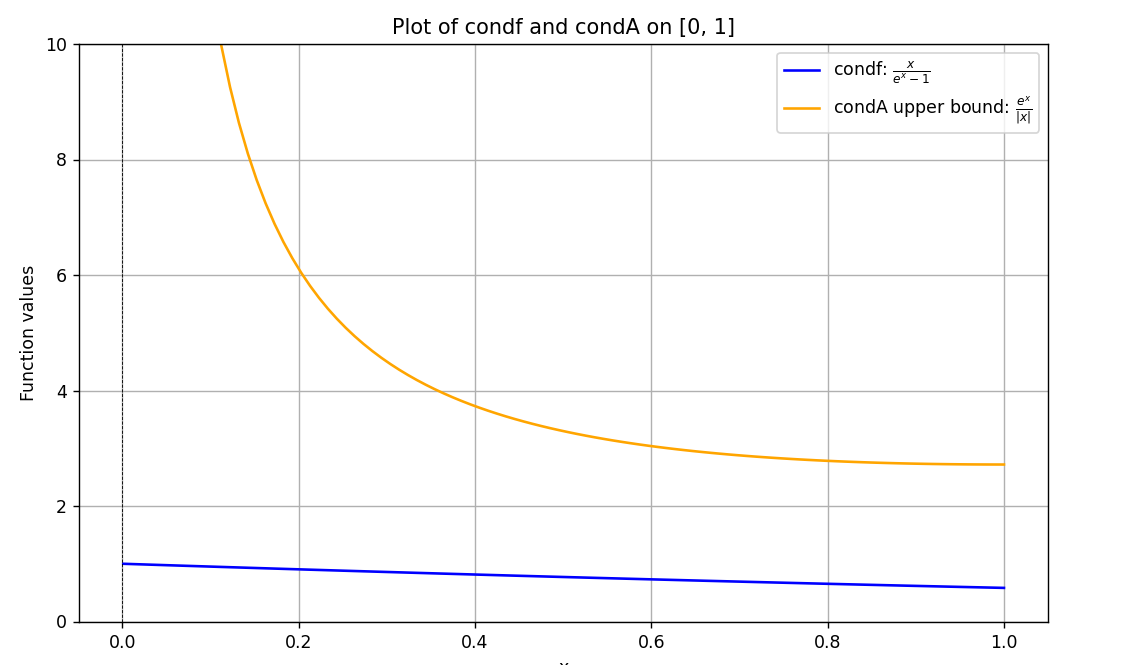
\includegraphics[width=0.8\textwidth]{plot.jpg}
  \caption{plot}
  \label{fig:condf}
\end{figure}

\section*{X}

   $\|\mathbf{A}\|_2 = \sup_{\|\mathbf{x}\|_2 = 1} \|\mathbf{A}\mathbf{x}\|_2$\\

   $\|\mathbf{A}^{-1}\|_2 = \sup_{\|\mathbf{y}\|_2 = 1} \|\mathbf{A}^{-1}\mathbf{y}\|_2$\\

Since $\mathbf{A}$ is a non-singular matrix, $\|\mathbf{A}^{-1}\|_2 < \infty$.\\

Do singular value decomposition on A, $A=U^T\Sigma V$, U, V are standard orthogonal arrays. Have $\sup_{\|\mathbf{x}\|_2 = 1} \|\mathbf{A}\mathbf{x}\|_2=\sup_{\|\mathbf{x}\|_2 = 1} \sqrt{x^TA^TAx}=\sup_{\|\mathbf{y}\|_2 = 1}\sqrt{y^T\Sigma^T\Sigma y}$\\
where $y=Vx$,\\
$\sqrt{y^T\Sigma^T\Sigma y} \leq \sqrt{\Sigma_{i=1}^n y_i^2\sigma_{i}^2} \leq \sqrt{(\Sigma_{i=1}^n y_i^2)\sigma_{max}^2}=\sigma_{max}$\\
To take the equal sign, just take the component of y corresponding to $\sigma_{max}$ as 1, the rest as 0, $x=V^{-1}y$ will do.\\
Do the same operation on $A^{-1}$, have\\
   $\|\mathbf{A^{-1}}\|_2 = \sigma_{\max}(A^{-1})=1/\sigma_{\min}$($\mathbf{A}$ is a square matrix, then its singular values are equal to the absolute values of the eigenvalues)\\

Therefore, the condition number $\text{cond}_2 \mathbf{A}$ can be expressed as:\\
   $\text{cond}_2 \mathbf{A} = \|\mathbf{A}\|_2 \|\mathbf{A}^{-1}\|_2 = \sigma_{\max}/\sigma_{\min}$\\

If $\mathbf{A}$ is a square matrix, then its singular values are equal to the absolute values of the eigenvalues. Therefore, we have:\\
   $\text{cond}_2 \mathbf{A} = |\lambda_{\max}|/|\lambda_{\min}|$\\

When A is an identity matrix, $|\lambda_{\max}|=|\lambda_{\min}|=1$\\
Therefore, $\text{cond}_2 \mathbf{A}=1$\\

In summary, the theorem is proved.\\

\section*{XI}
\[
\frac{\partial p}{\partial a_i} = r^i + p'(r) \frac{\partial r}{\partial a_i} = 0
\]
If \( p'(r) = 0 \), \( r^i = 0 \), and \( r = 0 \), combined with \( f(r) = 0 \), we obtain \( a_0 = 0 \), which leads to a contradiction. Therefore, \( p'(r) \neq 0 \).\\
\[
\frac{\partial r}{\partial a_i} = \frac{-r^i}{p'(r)}
\]
The condition number with respect to \( a_i \) is given by:\\
\[
\text{cond}_{f,a_i} = \frac{a_i \cdot \frac{-r^i}{p'(r)}}{r}
\]
Under the 1-norm, the condition number \( \text{cond}_f \) is:\\
\[
\left| \left( \frac{-a_0}{p'(r) \cdot r}, \frac{-a_1}{p'(r)}, \dots, \frac{-a_{n-1} \cdot r^{n-2}}{p'(r)} \right) \right|_1 = \max_{i=0..n-1} \left| \frac{-a_i \cdot r^{i-1}}{p'(r)} \right|
\]
For the Wilkinson example:\\
\[
f'(x) = \sum_{i=1}^p \prod_{k \neq i} (x - k)
\]
At \( f'(n) \), we have:
\[
f'(n) = \prod_{k \neq n} (x - k), \quad 0 \dots p
\]
Substituting this into the expression for the condition number:\\
\[
\text{cond}_f = \max_{n=0..p-1} \left| \frac{-(-1)^{p-n} \sigma_n(1,2,...,p) \cdot n^{i-1}}{\prod_{k \neq n} (n - k)} \right| = \max_{n=0..p-1} \left| \frac{\sigma_n(1,2,...,p) \cdot n^{i-1}}{\prod_{k \neq n} (n - k)} \right|
\]
The expression for the condition number of both cases is similar. However, in the Wilkinson example, the condition number changes drastically with perturbations, suggesting that similar equations will have large changes in their roots with perturbations.\\



\section*{XII}
Take 9-base under $p=2$ of $a=(1)_9,b=(7.7)_9$\\
$b/a=0.12857....$\\
In register $fl(a/b)=0.114$, result $fl(a/b)=1.2*9^{-1}$\\
$\frac{|\frac{fl(a/b)-a/b}{a/b}|}{\epsilon_u}=1.0123>1.$ Therefore, it does not conform to the formula\\

\section*{XIII}
No\\
For numbers a in [128,129]\\
$a=2^7*m_a,m_a\geq 1,a\leq 1+2^{-7}$\\
To achieve an absolute error less than 1e-6\\
Need to satisfy the two endpoints $x_R-x_L \leq (0.00000000000000000001)_2$\\
It is also known that $x_R,x_L\in [128,129]$, $x_R-x_L \geq 2^{1-24}*2^7>(0.00000000000000000001)_2$ contradiction\\

\section*{XIV}
Taking the linear system from Theorem 3.7 as an example:\\
\[
\begin{bmatrix}
  2 & \mu_2 & & & \\
  \lambda_3 & 2 & \mu_3 & & \\
  & \ddots & & \ddots & \\
  & \lambda_i & 2 & \mu_i & \\
  & & \ddots & & \\
  & & \lambda_{N-2} & 2 & \mu_{N-2} \\
  & & & \lambda_{N-1} & 2
  \end{bmatrix}
  \begin{bmatrix}
  m_2 \\
  m_3 \\
  \vdots \\
  m_i \\
  \vdots \\
  m_{N-2} \\
  m_{N-1}
  \end{bmatrix}
  =
  \mathbf{b}
\]
where \(\mu_i = \frac{x_i - x_{i-1}}{x_{i+1} - x_{i-1}}\) and \(\lambda_i = \frac{x_{i+1} - x_i}{x_{i+1} - x_{i-1}}\).\\
However, according to the Gershgorin Circle Theorem, the eigenvalues of the matrix are bounded within the interval [1,3], and the condition number is limited to the range [1,3], indicating good properties.\\
But if other construction methods are used, such as setting all coefficients as the objective for solving the linear system, and the interval between \(t_{i+1}\) and \(t_i\) is extremely small, situations like the following can occur:\\
The matrix for the cubic spline includes the positional relationships between adjacent data points. When the distance between two adjacent points is very small, it can cause some coefficients to approach zero, reducing the minimum singular value of matrix \( A \) and increasing its condition number.\\
\[ a_{i,1} + 2a_{i,2}\Delta + 3a_{i,n}\Delta^2 = a_{i+1,1} \]\\
\[ 2a_{i,2} + 6a_{i,3}\Delta = a_{i+2,1} \]\\

If \(\Delta\) is close to zero, it can cause the coefficients corresponding to \(a_{i,3}\) in the matrix to approach zero, making that column nearly a zero vector, which significantly increases the condition number. This can lead to large errors in the solution.\\


\section*{ \center{\normalsize {Acknowledgement}} }
Use GPT-4 for quick template transformation, and use Kimi AI to correct English grammar.

\end{document}
